\documentclass[12pt]{article} 

\usepackage[latin1]{inputenc}
\usepackage[spanish]{babel}
\usepackage{color}
\usepackage{multicol}
\usepackage{amsmath}
\usepackage{amssymb}
\usepackage{enumerate}
\usepackage{graphics}
\usepackage{graphicx}


\title{TREE SUMMING}
\author{Sara Chica, Rodrigo Gualtero}
\date{15 de Diciembre, 2012}

\begin{document}
\maketitle
\tableofcontents

\section{Introducci\'on}
Este es un problema de la UVA, identificado con el c\'odigo \textit{112}, El cual consiste en determinar si un n\'umero dado por el usuario corresponde a la suma de de las ramas de un \'arbol binario tambi\'en dado por el usuario.
\\A continuaci\'on se presenta un ejemplo en donde se puede observar un \'arbol binario dado por el usuario
\begin{center}
	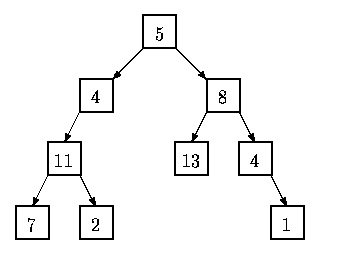
\includegraphics[width=0.50\textwidth]{mapa.jpg}
	\\El \'arbol es ingresado de la siguiente forma: (5 (4 (11 (7 () ()) (2 () ()) ) ()) (8 (13 () ()) (4 () (1 () ()) ) ) )
\end{center}

\section{Definici\'on del problema}
Para este problema la reprersentaci\'on m\'as adecuada es una estructira tipo \'arbol binario ya que cada uno de los \'arboles que ser\'an ingresados tienen dos ramas y estas a su vez tienen otras dos.
El objetivo de este ejercicio es determinar si un n\'umero dado por el usuario corresponde a la suma  de las ramas del \'arbol
\subsection{Entrada}
En un principio recibimos un entero \textit{N}  que corresponde a la suma de las ramas del arbol; a continuaci\'on se recibe una cadena de caracteres correspondiente al \'arbol, dentro de esta entrada se cuenta con dos tipos de caracteres el primero son caracteres de parentesis que indican si son ramas derechas o izquierdas del \'arbol y caracteres n\'umericos que se ubican en cada nodo del \'arbol.
\subsection{Salida}
Se debe imprimir la palabra  \textit{yes} o  \textit{not} si cumple o no con la suma correspondiente a las ramas del \'arbol
\section{Modelamiento Matem�tico}
Un �rbol binario es un �rbol en el que ning�n nodo puede tener m�s de dos sub�rboles. 
\\En este cada nodo puede tener cero, uno o dos hijos (sub�rboles), donde se conoce el nodo de la izquierda como hijo izquierdo y el nodo de la derecha como hijo derecho.
\\Estos cuentan con varios tipos de recorridos que permiten as� obtener informaci�n de ellos y manipularla; algunos de estos son: En profundidad, en preorden, en postorden, en inorden, por niveles, entre otros.
\section{Planteamiento de la Soluci\'on}
Para determinar la soluci\'on del problema primero se debe representar el la entrada como un \'arbol ; una vez hecho esto lo unico que se debe hacer es una busqueda por profundidad sacando en cada una de estas el valor que se encuentra en el nodo del \'arbol y poniendolo en un acomulador, al final se compara este n\'umero de acomulado con el n\'umero ingresado por el usuario; y si son iguales el resultado es yes de lo contrario es not.
\section{Conclusiones}
\begin{enumerate}
	\item La mejor forma para solucionar el problema es a trav\'es de un \'arbol ya que el ejercicio se vuelve muy simple cuando se ha armado el \'arbol.
	\item El problema es ideal para estudiantes que estan viendo recorridos en \'arboles y representacion de datos a trav\'es de \'arboles siempre y cuando la informaci\'on se represnte en \'arboles binarios.
\end{enumerate}
\end{document}